% \documentclass[fleqn,10pt]{wlscirep}
\documentclass{article}[11pt,oneside]
\usepackage[utf8]{inputenc}
\usepackage[T1]{fontenc}

\usepackage{amsrefs}
\makeatletter
\renewcommand{\BibLabel}{%
    \hfill
    \Hy@raisedlink{\hyper@anchorstart{cite.\CurrentBib}\hyper@anchorend}%
    \thebib.%
}
\makeatother
\renewcommand{\biblistfont}{%
  \normalfont
  \normalsize
}

\usepackage{authblk}

\usepackage[superscript,biblabel,nomove]{cite}

\newcommand{\edit}[1]{\textcolor{black}{#1}}
\newcommand{\newedit}[1]{\textcolor{black}{#1}}

\setlength{\paperwidth}{21cm}   % A4
\setlength{\paperheight}{29.7cm}% A4
\setlength\topmargin{-0.5cm}
\setlength\oddsidemargin{0cm}   
\setlength\textheight{24.7cm} 
\setlength\textwidth{16.5cm}
\setlength\columnsep{0.6cm}  

% custom packages
\usepackage{subcaption}
\usepackage{bm}
\usepackage{csquotes}
\usepackage{framed}
\usepackage{multicol}
\usepackage{changepage}
\usepackage{multirow}
\usepackage{setspace}
\usepackage{amsmath,amsfonts,amssymb,amsthm}
\usepackage{graphicx,xcolor}
\usepackage{booktabs}

%% Include all macros below

\newcommand{\dataset}{{\cal D}}
\newcommand{\fracpartial}[2]{\frac{\partial #1}{\partial  #2}}

\def\E{\mathbb{E}} % Expectation symbol
\def\Gsn{\mathcal{N}} % Normal distribution symbol
\def\Cov{\mrm{Cov}} % Covariance symbol
\def\reals{\mathbb{R}}
\newcommand{\capital}[1]{\bm{\mathrm{#1}}}
\renewcommand{\exp}[1]{\operatorname{exp}\left(#1\right)} % Exponential
\DeclareMathOperator*{\argmax}{argmax}
\DeclareMathOperator*{\argmin}{argmin}
\def\indic#1{\mbb{I}\left({#1}\right)} % Indicator function
\def\indicsub#1#2{\mbb{I}_{#2}\left({#1}\right)} % Indicator function

% TODO:
% 1. No footnote! 

\title{DeepTag: inferring diagnoses from veterinary clinical notes}

\author[1,+]{Allen Nie}
\author[1,+]{Ashley Zehnder}
\author[2]{Rodney L. Page}
\author[3]{Yuhui Zhang}
\author[1]{Arturo Lopez Pineda}
\author[1]{Manuel A. Rivas}
\author[1,4]{Carlos D. Bustamante}
\author[1,4, *]{James Zou}
\affil[1]{Department of Biomedical Data Science, Stanford University, Stanford, CA 94305, USA}
\affil[2]{Department of Clinical Sciences, Colorado State University, Fort Collins, CO 80523, USA}
\affil[3]{Department of Computer Science and Technology, Tsinghua University, Beijing, China}
\affil[4]{Chan-Zuckerberg Biohub, San Francisco, CA 94158, USA}

\affil[+]{these authors contributed equally to this work}
\affil[*]{Corresponding author. jamesz@stanford.edu}

\begin{document}

\maketitle

\begin{abstract}
Large scale veterinary clinical records can become a powerful resource for patient care and research. However, clinicians lack the time and resource to annotate patient records with standard medical diagnostic codes and most veterinary visits are captured in free text notes. The lack of standard coding makes it challenging to use the clinical data to improve patient care. 
It is also a major impediment to cross-species translational research, which relies on the ability to accurately identify patient cohorts with specific diagnostic criteria in humans and animals. In order to reduce the coding burden for veterinary clinical practice and aid translational research, we have developed a deep learning algorithm, DeepTag, which automatically infers diagnostic codes from veterinary free text notes. DeepTag is trained on a newly curated dataset of 112,558 veterinary notes manually annotated by experts.
DeepTag extends multi-task LSTM with an improved hierarchical objective that captures the semantic structures between diseases. To foster human-machine collaboration, DeepTag also learns to abstain in examples when it is uncertain and defers them to human experts, resulting in improved performance. DeepTag accurately infers disease codes from free text even in challenging cross-hospital settings where the text comes from different clinical settings than the ones used for training. It enables automated disease annotation across a broad range of clinical diagnoses with minimal pre-processing. The technical framework in this work can be applied in other medical domains that currently lack medical coding resources.
\end{abstract}

% \thispagestyle{empty}

% \noindent Please note: Abbreviations should be introduced at the first mention in the main text – no abbreviations lists. Suggested structure of main text (not enforced) is provided below.

% \doublespacing
\onehalfspacing

\section*{Introduction}

While a robust medical coding infrastructure exists in the US healthcare system for human medical records, this is not the case in veterinary medicine, which 
 lacks coding infrastructure and standardized nomenclatures across medical institutions. Most veterinary clinical notes are not coded with standard SNOMED-CT diagnosis~\cite{o2014approaches}. 
This hampers efforts at clinical research and public health monitoring. Due to the relative ease of obtaining large volumes of free-text veterinary clinical records for research (compared to similar volumes of human medical data) and the importance of turning these volumes of text into structured data to advance clinical research, we investigated effective methods for building automatic coding systems for the veterinary records. 

It is becoming increasingly accepted that spontaneous diseases in animals have important translational impact on the study of human disease for a variety of disciplines \cite{kol2015companion}. Beyond the study of zoonotic diseases, which represent 60-70\% of all emerging diseases, non-infectious diseases, like cancer, have become increasingly studied in companion animals as a way to mitigate some of the problems with rodent models of disease \cite{leblanc2016defining}. Additionally, spontaneous models of disease in companion animals are being used in drug development pipelines as these models more closely resemble the ``real world'' clinical settings of diseases than genetically altered mouse models~\cite{grimm2016bark,klinck2017translational,baraban2014new,hernandez2018naturally}. 
However, when it comes to identifying clinical cohorts of veterinary patients on a large scale for clinical research, there are several problems.  One of the first is that veterinary clinical visits rarely have diagnostic codes applied to them, either by clinicians or medical coders.  There is no substantial third party payer system and no HealthIT act that applies to veterinary medicine, so there are few incentives for clinicians or hospitals to annotate their records for diseases to be able to identify patients by diagnosis.  Billing codes are largely institution-specific and rarely applicable across institutions, unless hospitals are under the same management structure and records system. Some large corporate practice groups have their own internal clinical coding structures, but that data is rarely made available for outside researchers. A small number ($< 5$) academic veterinary centers (of a total of 30 veterinary schools in the US) employ dedicated medical coding staff that apply disease codes to clinical records so these records can be identified for clinical faculty for research purposes. How best to utilize this rare, well-annotated, veterinary clinical data for the development of tools that can help organize the remaining seqments of the veterinary medical domain is an open area of  research. 

In this paper, we develop DeepTag, a system to automatically code veterinary clinical notes. DeepTag takes free-form veterinary note as input and infers clinical diagnosis from the note. The inferred diagnosis is in the form of 42 SNOMED-CT codes. We trained DeepTag on a large set of 112,558 veterinary notes, and each note is expert labeled with a set of SNOMED-CT codes. DeepTag is a bidirectional long-short term memory network (BLSTM) augmented with a hierarchical training objective that captures similarities between the diagnosis codes. We evaluated DeepTag's performance on challenging cross-hospital coding tasks.

Natural language processing (NLP)  techniques have improved from leveraging discrete patterns such as n-grams \cite{jurafsky2014speech} to continuous learning algorithms like Long-short-term Memory Networks (LSTMs) \cite{hochreiter1997long}. This strategy has proven to be very successful when a sizable amount of data can be acquired. Combined with advances in optimization and classification algorithms, the field has developed algorithms that can match or exceed human performance in several traditionally difficult tasks \cite{goldberg2017neural}.

Analyzing free text such as diagnostic reports and clinical notes has been a central focus of clinical natural language processing~\cite{velupillai2015recent}. Most of the previous research has focused on the human healthcare systems. Examples include using NLP tools to improve pneumonia screening in the emergency department, assisting in adenoma detection, assisting and simplifying hospital processes by identifying billing codes from clinical notes~\cite{demner2016aspiring}. Pivovarov et al. have conducted experiments to discover phenotypes and diseases using an unsupervised method on a broad set of heterogeneous data~\cite{pivovarov2015learning}.

In the domain of veterinary medicine, millions of clinical summaries are stored as electronic health records (EHR) in various hospitals and clinics. Unlike human discharge summaries that have been assigned with billing codes (ICD-9/ICD-10 codes), veterinary summaries exist primarily as free text. This makes it challenging to perform  systematic analysis  such as disease prevalence studies, analysis of adverse drug effects, therapeutic efficacy or outcome analysis. Veterinary domain is very favorable for an NLP system that can convert large amount of  free-text notes into structured information. Such a system would benefit the veterinary community in a substantial way and can be deployed in multiple clinical settings. Veterinary medicine is a domain where clinical NLP tools can have a substantial impact in practice and be integrated into daily use.

Identifying a set of conditions/diseases from clinical notes has been actively studied~\cite{demner2016aspiring,lipton2015learning}. Currently, the task of transforming free text into structured information primarily relies on two approaches: named entity recognition (NER) and automated coding. DeepTag is designed to perform automated coding rather than NER. NER requires annotation on the word level, where each word is associated with one of a few types. In the ShARe task \cite{pradhan2014evaluating}, the importance is placed on identifying disease span and then normalizing into standard terminology in SNOMED-CT or UMLS (Unified Medical Language System). In other works, the focus has been on tagging each word with a specific type: adverse drug effect, severity, drug name, etc~\cite{jagannatha2016bidirectional}. Annotating on word level is expensive, and most corpora contain only a couple of hundreds or thousands of clinical notes. Even though early shared task in this domain has proven to be successful  ~\cite{pradhan2014semeval,elhadad2015semeval}, it is still difficult to curate a large dataset in this manner.

Automated coding on the other hand takes the entire free text as input, and infers a set of codes that are used to code the entire work. Most discharge summaries in human hospitals have billing codes assigned. Baumel et al. proposed a text processing model for automated coding that processes each sentence first and then processes the encoded hidden states for the entire document~\cite{baumel2017multi}.This multi-level approach is especially suitable for longer texts, and the method was applied to the MIMIC data, where each document is on average five times longer than the veterinary notes from CSU. Rajkomar et al. used deep learning methods to process the entire EHR and make clinical predictions for a wide range of problems including automated coding~\cite{rajkomar2018scalable}. In their work, they compared three deep learning models: LSTM, time-aware feedforward neural network (TANN), and boosted time-based decision stumps. In this work, we use a new hierarchical training objective which is designed to capture the similarities among the SNOMED-CT codes. This hierarchical objective is complementary to these previous approaches in the sense that the hierarchical objective can be used on top of any architecture. Our cross-hospital evaluations also extend what is typically done in literature. Even though Rajkomar et al. had data from two hospitals, they did not investigate the performance of the model when trained on one hospital but evaluated on the other. In our work, due to the lack of coded clinical notes in the veterinary community beyond a few academic hospitals, it is especially salient for us to evaluate the model’s ability to generalize across hospitals.

Our work is also related to the work of Kavuluru et al., who experimented with different training strategies and compared which strategy is the best for automated coding~\cite{kavuluru2015empirical}, and Subotin et al., who improved upon direct label probability estimation and used a conditional probability estimator to fine-tune the label probability~\cite{subotin2016method}. Perotte et al. also investigated possible methods to leverage the hierarchical structure of disease codes by using an SVM algorithm on each level of the ICD-9 hierarchy tree~\cite{perotte2013diagnosis}.

Cross-hospital generalization is a significant challenge in the veterinary coding setting. Most veterinary clinics currently do not apply diagnosis codes to their notes~\cite{o2014approaches}. Therefore our training data can only come from a handful of university-based regional referral centers that manually code their free text notes. The task is to train a model on such data and deploy for thousands of private hospitals and clinics. University-based centers and private hospitals and clinics have substantial variation in the writing style, the patient population, and the distribution of diseases (Figure~1). For example, the training dataset we have used in this work comes from a university-based hospital with a high-volume referral oncology service, but typical local hospitals might face more dermatologic or gastrointestinal cases.

\section*{Results}

DeepTag takes clinician's notes as input and predicts a set of SNOMED-CT disease codes. SNOMED-CT is a comprehensive and precise clinical health terminology managed by the International Health Terminology Standards Development Organization. DeepTag is a bi-directional long short-term memory (LSTM) neural network with a new hierarchical learning objective designed to
capture similarities between the disease codes (see the Supplement for model details). 

DeepTag is trained on 112,558 annotated veterinary notes from the Colorodo State University of Veterinary Medicine and Biomedical Sciences (CSU) curated for research purposes. Each of these notes is a free text description of a patient visit, and is manually tagged with at least one, and on average eight, out of the 41 SNOMED-CT disease codes by experts. 
In addition, we map every non-disease related code to an extra  code. In total, DeepTag learns to tag a clinical note with a subset of 42 codes.
 
We evaluate DeepTag on two different datasets. One consists of 5,628 randomly sampled non-overlapping held-out documents from the same CSU dataset that the system is trained on. The other dataset contains 586 documents and are collected from a private practice (PP) located in northern California. Each of the these document is also manually annotated with the appropriate SNOMED-CT codes by human experts. We refer to this dataset as the PP dataset. 

We regard the PP dataset as a ``out-of-domain'' dataset due to its substantial difference with regard to writing style and institution type compared to the CSU dataset~\cite{li2012literature}. The PP documents tend to be substantially shorter (average of 253 words compared to 368 words in CSU), use more abbreviations and have different distribution of diseases (see Methods section for more details).
 
\subsection*{Tagging performance}

We present DeepTag's performance on the CSU and PP test data in Table~1. To save space, we display the 20 most frequent disease codes in Table~1. For each disease code, we report the number of training examples for the disease code ($N$), the scores for precision, recall, $F_1$, ROC AUC, and the number of subtypes in this disease code. While DeepTag achieves reasonable $F_1$ scores overall, its performance is quite heterogeneous for different disease codes. Moreover, the performance decreases when DeepTag is applied to the out-of-domain PP test data. 
We identify two factors that substantially impact DeepTag's performance: 1) the number of training examples that are tagged with the given disease code; 2) the number of subtypes, where a subtype is a SNOMED-CT code applied to either dataset that is lower in the SNOMED-CT hierarchy than the top-level disease codes DeepTag is predicting. We use the number of subtypes as a proxy for the diversity and specificity of the clinical text descriptions. Thus, a higher number of subtypes suggests a wider spectrum of diseases.

\paragraph{Performance improves with more training examples.}
We first note that DeepTag works relatively well when the number of training examples for each disease code is abundant. We generate a scatter plot to capture the correlation between number of examples in the in CSU dataset and the disease code's $F_1$ score evaluated on the CSU test set. We also plot the $F_1$ score for the disease code evaluated on the PP dataset and its number of training examples on the CSU dataset. 

For the CSU dataset, we observe an almost linear relationship between the log number of examples and the $F_1$ score in Figure~2, suggesting that our large training data is crucial for the prediction performance. 
We observe a similar pattern when evaluating on the PP dataset, thought the correlation is weaker and the pattern is less linear. This is due to the out-of-domain nature of PP, which we investigate in depth below.

\paragraph{More diverse disease codes are harder to predict.}
After observing the general correlation between number of training examples and per-disease code $F_1$ scores, we can investigate outliers. These are diseases that have many examples but on which DeepTag performed poorly and diseases that have few examples but DeepTag performed well. For \emph{disorder of digestive system}, despite having the second highest number of training examples (22,589), both precision and recall are lower than other frequent diseases. We find that this disease code covers the second largest number of subtypes (694). On the other hand, \emph{disorder of hematopoietic cell proliferation} has the highest $F_1$ score with relatively few training examples ($N = 7294$). This disease code has only 22 subtypes. Similarly \emph{autoimmune diseases} has  few training examples ($N = 1280$) but it still has a relatively high $F_1$, and it also has only 11 subtypes.

The number of subtypes---i.e. the number of different lower level SNOMED-CT codes that are mapped to each of the 42 higher-level disease code---can serve as an indicator for the diversity or specificity of the text descriptions. For a disease like \emph{disorder of digestive system}, it subsumes many different types of diseases such as \emph{periodontal disease}, \emph{hepatic disease}, and \emph{disease of stomach}, which all have
different diagnoses. Similarly, \emph{Neoplasm and/or hamartoma} encapsulates many different histologic types and be categorized as benign, malignant, or unknown, thus resulting in many different lower-level  codes (749 codes) being mapped into the same top-level disease code. DeepTag needs to associate diverse descriptions to the same high-level disease code, increasing the difficulty of the prediction task.

We hypothesize that disease codes with many subtypes will be difficult for the system to predict. This hypothesis suggests that the number of subtypes a disease code contains could explain some of the heterogeneity in DeepTag's performance beyond the heterogeneity due to the training sample size.

We conduct a multiple linear regression test with both the number of training examples as well as number of subtypes each disease code contains as covariates and the $F_1$ score as the outcome. In the regression, the coefficient for number of subtypes is negative with $p < .001$. This indicates that, controlling for the number of training examples, having more subtypes in a disease code makes tagging more challenging and decreases DeepTag's performance on the disease code.

\paragraph{Performance on PP}

Next we investigate DeepTag's performance discrepancy between the CSU and PP test data. A primary contributing factor to the discrepancy is that the underlying text in PP is stylistically and functionally different from the text in CSU. Note that DeepTag was only trained on the CSU text and was not fine-tuned on PP. The example texts in Figure~1 illustrate the striking difference. In particular, PP uses many more abbreviations that are not observed in CSU.

After filtering out numbers, 15.4\% of words in PP are not found in CSU. Many of the PP specific words appear to be medical acronyms that are not used in CSU or terms that describe test results or medical procedures. Since these vocabulary has no trained word embedding from the CSU dataset, DeepTag can not leverage them in the disease tagging process. 

Despite having many training examples, DeepTag performs poorly on some very frequent diseases, for example, \emph{neoplasm and/or hamartoma}. 
On the opposite end of the spectrum, the tagger does well for \emph{disorder of auditory system} on both CSU and PP dataset, despite only having a moderate amount of training examples. Besides the main issue of vocabulary mismatch, many subtypes (lower-level disease codes) that get mapped to a disease code in CSU do not exist in PP, and subtypes in PP also might not exist in CSU. We refer to this as the subtype distribution shift.
For example, In CSU, \emph{neoplasm and/or hamartoma} has 749 observed subtypes. Only 7 out of 749 subtypes are present in PP. Moreover, there are 11 subtypes are unique to the PP dataset and are not observed in the CSU training set. 

In addition to the subtype analysis, we note that for rarer diseases, the precision drop between CSU and PP is not as deep as the recall drop. This can be interpreted as the model is fairly confident and precise about the key phrases it discovered from the CSU dataset. The drop in recall in the PP dataset could be partially due the fact that PP uses many terms and phrases that are not in the CSU data.

\subsection*{Improvements from disease similarity}
The 42 disease codes can be naturally grouped into 18 meta-diseases; each meta-disease corresponds to a subset of diseases that are related to each other (see the Supplement). For example, the disease codes for ``Disease caused by Arthropod'' and ``Disease caused by Annelida'' belong to the same meta-disease, ``Infectious and parasitic diseases''. We designed DeepTag to leverage this hierarchical structure amongst the disease codes. Intuitively, suppose the true disease associated with a note is $A$ and DeepTag mistakenly predicts disease code $B$. Then its penalty should be larger if $B$ is very different from $A$---i.e., they are in different meta-diseases---than if $B$ and $A$ are in the same meta-disease. More precisely, we use the grouping of similar codes into meta-diseases as a regularization in the training objective of DeepTag. Basic deep learning systems like LSTM and BLSTM do not incorporate this information.

DeepTag uses a $L_2$-based distance objective to place this constraint between disease code embeddings, which are the parameters in the final layer of the DeepTag neural network. The objective encourages the embeddings of disease codes that are in the same meta-disease to be closer to each other than the embeddings of disease codes across different meta-diseases. In addition, we investigated another approach that can also leverage disease similarity: DeepTag-M. This method computes the probability of a meta-disease based on the probability of the disease codes that are grouped into it. Instead of forcing similarity constraints on disease code embeddings, DeepTag-M encourages the model to make correct prediction on the meta-diseases as well as on the disease codes (see the Supplement).

In Table~2, we compare the performance of DeepTag and DeepTag-M with the standard multi-task LSTM, bidirectional LSTM (BLSTM), text convolutional neural network (CNN), MetaMap-SVM and MetaMap-MLP. MetaMap is a non-deep learning approach that processes each document to extract a set of medically-relevant terms \cite{aronson2010overview}. We then train a support vector machine (MetaMap-SVM) or a multi-layer perceptron (MetaMap-MLP) to use the extracted terms to predict disease codes.

On the CSU dataset, DeepTag and DeepTag-M perform slightly better  compared to the baseline deep learning models (CNN, LSTM and BLSTM). All the deep learning models performed substantially better than MetaMap-SVM and MetaMap-MLP on CSU. DeepTag has higher unweighted precision, recall, and $F_1$ score compared to the other models, indicating its ability to have good performance on a wide spectrum of diseases. The importance of leveraging similarity is shown on the PP dataset (Figure~3).  Since it is out-of-domain, expert defined disease similarity provide much-needed regularization to make both DeepTag and DeepTag-M outperform baseline models by a substantial margin, with DeepTag being the overall best model. 

\subsection*{Learning to abstain}

Augmenting a tagging system with the ability to abstain (decline to assign codes) can foster human-machine collaboration. When the system does not have enough confidence to make decisions, it has the option to defer to its human counterparts. This aspect is important in DeepTag because after tagging the documents, further analysis from various parties might be conducted on the tagged documents such as investigating the prevalence of certain specific diseases. In order to not mislead further clinical research, having the ability to abstain from making very erroneous predictions and ensuring highly precise tagging is an important feature.

A natural approach to decide whether to abtain on a given document is to check whether the DeepTag prediction confidence---i.e. the output of the final logistic regression---is above a set threshold. We use this approach as the baseline abstention method. This could be suboptimal if DeepTag is over-confident in its predictions. Therefore, we also developed an additional abstention wrapper on top of DeepTag that we call DeepTag-abstain. DeepTag-abstain takes the prediction confidence of the original DeepTag for each of the 42 codes and learns a non-linear function in order to decide whether to abstain. This learning to abstain approach gives DeepTag-abstain more flexibility to assess the multi-label prediction confidence. See the Supplement for more details about DeepTag-abstain and the baseline.

In order to evaluate how well DeepTag-abstain performs compared to the baseline, we compute an abstention priority score for each document. A document with higher abstention priority score will be removed earlier than a document with lower score. We then compute the weighted average of $F_1$ and exact match ratio (EM) for all the documents that are not removed.

For both baseline and DeepTag-abstain, we specify a proportion of the documents that need to be removed. We adjust the dropped portion from 0 to 0.9 (dropping 90\% of the examples at the high end). An abstention method that can drop more erroneously tagged documents earlier will observe a faster increase in its performance, corresponding to a curve with steeper slope. 

DeepTag-abstain demonstrates a substantial improvement over the baseline in Figure~4. 
We note that not all learning to abstain schemes are able to out-perform the baseline. The details of module design and improvement curve for the rest of the modules can be seen in the Supplemental Figure~2.

\section*{Discussion}

In this study, we developed a multi-label classification algorithm for veterinary clinical text, which represents a medical domain with an under-resourced medical coding infrastructure. In order to improve the performance of DeepTag on diseases with rare occurrences, we investigated with loss augmentation strategies that leverage the similarity and dissimilarity between the disease codes. These augmentations provide gains over the LSTM and BLSTM baselines, which are common methods used for these types of prediction tasks. We also experimented with different methodologies to allow the model to learn to abstain on examples where the model is not confident in the predictions. We demonstrate that learned abstention rules outperform manually set rules.

Our work demonstrates novel methods for applying broad disease codes to clinical records as well as applying those trained algorithms to an external dataset in order to examine cross-hospital generalization. We also demonstrate means to allow human domain experts to use their judgment when automated taggers have a high level of uncertainty in order to improve the overall workflow. We confirm that cross-hospital generalization is a significant concern for learned tagging systems to be deployed in real world implementations that may vary substantially from the data on which they were trained. 
Even though our work attempts to mitigate this problem, there is significant research to be done to optimize methods for domain adaptation.
Our current work is important not only for veterinary medical records, which are rarely coded, but also may have implications for human medical records in countries with limited coding infrastructure and which are important regions of the world for public health surveillance and clinical research. 

There are several aspects of the data that may have limited our ability to apply methods from our training set to our external validation set. Private veterinary practices often have data records that closely resemble the PP dataset used to evaluate our methods here. However, the large annotated dataset we used for training is from an academic institution (as these are, largely, the institutions that have dedicated medical coding staff). As can be seen from Table~2, the performance drop due to domain mismatch is non-negligible. The domain shift comes from two parts. First, text style mismatch -- private commercial notes use more abbreviations and tend to include many procedural examinations (even though many are non-informative or non-diagnostic). 

Second, disease code distribution mismatch -- the CSU training dataset focuses largely on neoplasm and several other tumor-related diseases, largely due to the fact that the CSU hospital is a regional tertiary referral center for cancer and cancer represents nearly 30\% of the caseload. Other practices will have datasets composed of disease codes that appear with different frequencies, depending on the specializations of that particular practice. A very important path forward is to use learning algorithms that are robust to domain shift, and experimenting with unsupervised representation learning to mitigate the domain shift between academic datasets and private practice datasets.

Currently we are predicting top-level SNOMED-CT disease codes, which are not the SNOMED-CT codes that have been directly annotated on the dataset. Many of the SNOMED-CT codes that are applied to clinical records are coded as 'Findings' that are not actual 'Disorders' as the actual diagnosis of a patient may not be clear at the time the codes are applied.  One example is an animal that is evaluated for 'vomiting' and the actual cause is not determined, may have a code of 'vomiting(finding)'(300359004) applied and not 'vomiting(disorder)'(422400008) and these 'non-disorder' disease codes are not evaluated in our current work.  However, these are an important subset of codes and represent another means to identify particular patient cohorts with particular clinical signs or presentations, vs. diagnosed disorders. 

Another future direction for the abstention branch of this work is to factor human cost and annotation accuracy into the model and only defer when the model believes that human experts will bring improvement to the result within an acceptable amount of cost. This is an interesting direction for experimentation.

\section*{Methods}

\subsection*{Datasets}

\paragraph{Colorado State University dataset}
The CSU dataset contains discharge summaries as well as applied diagnostic codes for clinical patients from the Colorado State University College of Veterinary Medicine and Biomedical Sciences. 
This institution is a tertiary referral center with an active and nationally recognized cancer center. Because of this, the CSU dataset over-represents cancer-related diseases. Rare diseases in the CSU dataset are diseases like  perinatal and mental disorders, but these are also rare in the larger veterinary population as a whole and do not represent a dataset bias. Overall, there are 112,558 unique discharge summaries in CSU dataset.  We split this dataset into training, validation, and test set by 0.9/0.05/0.05. 

\paragraph{Private Practice dataset}
An external validation dataset was obtained from a regional private practice (PP).  These records did not have diagnostic codes available and only approximately 3\% of these records had a diagnosis placed in the ``Problem List'' for a particular patient on a particular visit. Out of 352,597 patient records obtained that had SOAP notes (i.e. notes in the ``Subjective, Objective, Assessment, Plan'' format), only 13843 (3.9\%) had at least one specific clinical diagnosis listed in the problem list.  These diagnoses were free text and not coded to SNOMED-CT by the primary clinicians.  Within the SOAP notes, additional diagnoses were frequently found within the “Assessment” field, but were not applied in a consistent standard and by using different levels of evidence, i.e., some of these diagnosis were presumptive, tentative or historical.

Two veterinary domain experts applied SNOMED-CT codes to a subset of these records and achieved consensus on the records used for validation. This dataset (PP) is used for external validation of algorithms developed using the CSU dataset. There are 586 documents in this external validation dataset.

\subsection*{Data processing}

Documents in our corpus have been tagged with SNOMED-CT codes that describe the clinical conditions present at the time of the visit being annotated.  Annotations are applied from the SNOMED-CT veterinary extension (SNOMEDCT\_VET), which is fully compatible to and is an extension of the International SNOMED-CT edition.  It can be accessed in a dedicated browser and is maintained by the Veterinary Terminology Services Laboratory at the Virginia-Maryland Regional College of Veterinary Medicine.  Medical coders applying diagnostic codes are either veterinarians or trained medical coders with expertise in the veterinary domain and the SNOMED terminology. The medical coding staff at CSU utilize post-coordinated expressions, where required, for annotations to fully describe a diagnosed condition. For this work, we only considered the core disease codes and not the subsequent modifiers for training our models.  The PP dataset was similarly coded using post-coordinated terms following consultation with coding staff at multiple academic institutions that annotate records using SNOMED-CT. We further grouped the 42 disease codes into 18 meta-diseases. More details of this grouping are provided in the Supplement.

\subsection*{Difference in data structures}
Due to the inherent differences in clinical notes/discharge summaries prepared for patients in an academic setting compared to the shorter `SOAP' format notes (Subjective, Objective, Assessment, Plan) prepared in private practice, there are substantial differences in the format as well as the writing style and level of detail between these two datasets. In addition, the private practice records exhibit significant differences in record styles between clinicians, as some clinicians use standardized forms while others use abbreviated clinical notes containing only references to abnormal clinical findings. 

As can be seen in Supplemental Figure~1, both dataset have more than 80\% documents associated with more than one disease code, and in terms of document length distribution, PP dataset document is much shorter than CSU dataset, while the average PP document length is 191 words. The average CSU document length is 325 words.

\subsection*{Algorithm development and analysis}

We trained our modeling algorithm on CSU dataset and evaluated on a held-out portion of data from the CSU dataset as well as the PP dataset. 
We formulated our base model to be a recurrent neural network with long short-term memory cells (LSTM). We additionally decided to run this recurrent neural network on both the forward direction and backward direction of the document (bidrectional), as is found beneficial in Graves et al. \cite{graves2005bidirectional}. We then built 42 independent binary classifiers to predict the existence of each disease code. This is the architecture found most useful in multi-label classification literature \cite{kavuluru2015empirical}. The model is trained jointly with binary cross entropy loss. We then augmented this baseline model with two losses: cluster penalty \cite{jacob2009clustered} and a novel meta-disease prediction loss to leverage human expert knowledge in how semantically related these disease codes are.

\section*{Data availability}
The data that support the findings of this study are available from Colorado State University College of Veterinary Medicine and a private practice veterinary hospital near San Francisco, but restrictions apply to the availability of these data,
which were made available to Stanford for the current study, and so are not publicly available. Data are however available from the authors upon
reasonable request and with permission of Colorado State University College of Veterinary Medicine and the private hospital.

\section*{Code availability}
DeepTag is freely available at \url{https://github.com/windweller/DeepTag}.

\section*{Acknowledgements}

We would like to acknowledge the help of Devin Johnsen for her help in annotating the private practice records used in this work. We also want to thank Selina Dwight and Matthew Wright for helpful feedback. 
Our work is funded by the Chan-Zuckerberg Investigator Program and  National Science Foundation (NSF) Grant CRII 1657155.

\section*{Author contributions statement}

A.N. and A.Z. share co-first authorship. A.N. performed the natural language processing work, designed and built DeepTag and DeepTag-abstain, performed all the experiments, and analyzed the overall system's performance.  A.Z. acquired the data, established the meta-disease hierarchy, organized and aided in annotation of the private practice data, and provided feedback on the NLP and machine learning outputs. R.P. provided access to the training data. A.P. aided in initial data acquisition and used MetaMap software to generate features. Y.Z. ran MLP and SVM algorithms on the MetaMap features generated by A.P. M.R. and C.B. provided feedback on the project. J.Z. designed and supervised the project. A.N., A.Z. and J.Z. wrote the paper.

\section*{Additional information}
\textbf{Competing Interests}: the authors declare no competing interests.

% \bib, bibdiv, biblist are defined by the amsrefs package.
\begin{bibdiv}
\begin{biblist}

\bib{aronson2010overview}{article}{
      author={Aronson, Alan~R},
      author={Lang, Fran{\c{c}}ois-Michel},
       title={An overview of metamap: historical perspective and recent
  advances},
        date={2010},
     journal={Journal of the American Medical Informatics Association},
      volume={17},
      number={3},
       pages={229\ndash 236},
}

\bib{baraban2014new}{incollection}{
      author={Baraban, Scott~C},
      author={L{\"o}scher, Wolfgang},
       title={What new modeling approaches will help us identify promising drug
  treatments?},
        date={2014},
   booktitle={Issues in clinical epileptology: A view from the bench},
   publisher={Springer},
       pages={283\ndash 294},
}

\bib{baumel2017multi}{inproceedings}{
      author={Baumel, Tal},
      author={Nassour-Kassis, Jumana},
      author={Cohen, Raphael},
      author={Elhadad, Michael},
      author={Elhadad, Nóemie},
       title={Multi-label classification of patient notes: Case study on icd
  code assignment},
        date={2018},
   booktitle={Aaai workshops},
         url={https://aaai.org/ocs/index.php/WS/AAAIW18/paper/view/16881},
}

\bib{demner2016aspiring}{article}{
      author={Demner-Fushman, D},
      author={Elhadad, Noemie},
       title={Aspiring to unintended consequences of natural language
  processing: a review of recent developments in clinical and
  consumer-generated text processing},
        date={2016},
     journal={Yearbook of medical informatics},
      number={1},
       pages={224},
}

\bib{elhadad2015semeval}{inproceedings}{
      author={Elhadad, No{\'e}mie},
      author={Pradhan, Sameer},
      author={Gorman, Sharon},
      author={Manandhar, Suresh},
      author={Chapman, Wendy},
      author={Savova, Guergana},
       title={Semeval-2015 task 14: Analysis of clinical text},
        date={2015},
   booktitle={Proceedings of the 9th international workshop on semantic
  evaluation (semeval 2015)},
       pages={303\ndash 310},
}

\bib{goldberg2017neural}{article}{
      author={Goldberg, Yoav},
       title={Neural network methods for natural language processing},
        date={2017},
     journal={Synthesis Lectures on Human Language Technologies},
      volume={10},
      number={1},
       pages={1\ndash 309},
}

\bib{graves2005bidirectional}{inproceedings}{
      author={Graves, Alex},
      author={Fern{\'a}ndez, Santiago},
      author={Schmidhuber, J{\"u}rgen},
       title={Bidirectional lstm networks for improved phoneme classification
  and recognition},
organization={Springer},
        date={2005},
   booktitle={International conference on artificial neural networks},
       pages={799\ndash 804},
}

\bib{grimm2016bark}{misc}{
      author={Grimm, David},
       title={From bark to bedside},
   publisher={American Association for the Advancement of Science},
        date={2016},
}

\bib{hernandez2018naturally}{article}{
      author={Hernandez, Belen},
      author={Adissu, Hibret~A},
      author={Wei, Bih-Rong},
      author={Michael, Helen~T},
      author={Merlino, Glenn},
      author={Simpson, R~Mark},
       title={Naturally occurring canine melanoma as a predictive comparative
  oncology model for human mucosal and other triple wild-type melanomas},
        date={2018},
     journal={International journal of molecular sciences},
      volume={19},
      number={2},
       pages={394},
}

\bib{hochreiter1997long}{article}{
      author={Hochreiter, Sepp},
      author={Schmidhuber, J\"urgen},
       title={Long short-term memory},
        date={1997},
     journal={Neural computation},
      volume={9},
      number={8},
       pages={1735\ndash 1780},
}

\bib{jacob2009clustered}{inproceedings}{
      author={Jacob, Laurent},
      author={Vert, Jean-philippe},
      author={Bach, Francis~R},
       title={Clustered multi-task learning: A convex formulation},
        date={2009},
   booktitle={Advances in neural information processing systems},
       pages={745\ndash 752},
}

\bib{jagannatha2016bidirectional}{inproceedings}{
      author={Jagannatha, Abhyuday~N},
      author={Yu, Hong},
       title={Bidirectional rnn for medical event detection in electronic
  health records},
organization={NIH Public Access},
        date={2016},
   booktitle={Proceedings of the conference. association for computational
  linguistics. north american chapter. meeting},
      volume={2016},
       pages={473},
}

\bib{jurafsky2014speech}{book}{
      author={Jurafsky, Dan},
      author={Martin, James~H},
       title={Speech and language processing},
   publisher={Pearson London:},
        date={2014},
      volume={3},
}

\bib{kavuluru2015empirical}{article}{
      author={Kavuluru, Ramakanth},
      author={Rios, Anthony},
      author={Lu, Yuan},
       title={An empirical evaluation of supervised learning approaches in
  assigning diagnosis codes to electronic medical records},
        date={2015},
     journal={Artificial intelligence in medicine},
      volume={65},
      number={2},
       pages={155\ndash 166},
}

\bib{kim2014convolutional}{inproceedings}{
      author={Kim, Yoon},
       title={Convolutional neural networks for sentence classification},
        date={2014},
   booktitle={Proceedings of the 2014 conference on empirical methods in
  natural language processing (emnlp)},
       pages={1746\ndash 1751},
}

\bib{klinck2017translational}{article}{
      author={Klinck, Mary~P},
      author={Mogil, Jeffrey~S},
      author={Moreau, Maxim},
      author={Lascelles, B Duncan~X},
      author={Flecknell, Paul~A},
      author={Poitte, Thierry},
      author={Troncy, Eric},
       title={Translational pain assessment: could natural animal models be the
  missing link?},
        date={2017},
     journal={Pain},
      volume={158},
      number={9},
       pages={1633\ndash 1646},
}

\bib{kol2015companion}{article}{
      author={Kol, Amir},
    author={Arzi, Boaz},
      author={Athanasiou, {Kyriacos A}},
           author={Farmer, {Diana L}},
      author={Nolta, {Jan A}},
    %   author={Rebhun, {Robert B}},
    %   author={Chen, Xinbin},      
    %   author={Griffiths, {Leigh G}},
    %   author={Murphy, {Christopher J}},
    %   author={Verstraete, {Frank JM}},
      author={others},
       title={Companion animals: Translational scientist’s new best friends},
        date={2015},
     journal={Science translational medicine},
      volume={7},
      number={308},
       pages={308ps21\ndash 308ps21},
}

\bib{leblanc2016defining}{article}{
      author={LeBlanc, Amy~K},
      author={Mazcko, Christina~N},
      author={Khanna, Chand},
       title={Defining the value of a comparative approach to cancer drug
  development},
        date={2016},
     journal={Clinical Cancer Research},
      volume={22},
      number={9},
       pages={2133\ndash 2138},
}

\bib{li2012literature}{article}{
      author={Li, Qi},
       title={Literature survey: domain adaptation algorithms for natural
  language processing},
        date={2012},
     journal={Department of Computer Science The Graduate Center, The City
  University of New York},
       pages={8\ndash 10},
}

\bib{lipton2015learning}{inproceedings}{
      author={Lipton, Zachary~C},
      author={Kale, David~C},
      author={Elkan, Charles},
      author={Wetzel, Randall},
       title={Learning to diagnose with lstm recurrent neural networks},
        date={2016},
   booktitle={International conference on learning representations},
}

\bib{o2014approaches}{article}{
      author={O’Neill, Dan~G},
      author={Church, David~B},
      author={McGreevy, Paul~D},
      author={Thomson, Peter~C},
      author={Brodbelt, Dave~C},
       title={Approaches to canine health surveillance},
        date={2014},
     journal={Canine genetics and epidemiology},
      volume={1},
      number={1},
       pages={2},
}

\bib{perotte2013diagnosis}{article}{
      author={Perotte, Adler},
      author={Pivovarov, Rimma},
      author={Natarajan, Karthik},
      author={Weiskopf, Nicole},
      author={Wood, Frank},
      author={Elhadad, No{\'e}mie},
       title={Diagnosis code assignment: models and evaluation metrics},
        date={2013},
     journal={Journal of the American Medical Informatics Association},
      volume={21},
      number={2},
       pages={231\ndash 237},
}

\bib{pivovarov2015learning}{article}{
      author={Pivovarov, Rimma},
      author={Perotte, Adler~J},
      author={Grave, Edouard},
      author={Angiolillo, John},
      author={Wiggins, Chris~H},
      author={Elhadad, No{\'e}mie},
       title={Learning probabilistic phenotypes from heterogeneous ehr data},
        date={2015},
     journal={Journal of biomedical informatics},
      volume={58},
       pages={156\ndash 165},
}

\bib{pradhan2014semeval}{inproceedings}{
      author={Pradhan, Sameer},
      author={Elhadad, No{\'e}mie},
      author={Chapman, Wendy},
      author={Manandhar, Suresh},
      author={Savova, Guergana},
       title={Semeval-2014 task 7: Analysis of clinical text},
        date={2014},
   booktitle={Proceedings of the 8th international workshop on semantic
  evaluation (semeval 2014)},
       pages={54\ndash 62},
}

\bib{pradhan2014evaluating}{article}{
      author={Pradhan, Sameer},
      author={Elhadad, No{\'e}mie},
      author={South, Brett~R},
      author={Martinez, David},
      author={Christensen, Lee},
      author={Vogel, Amy},
      author={Suominen, Hanna},
      author={Chapman, Wendy~W},
      author={Savova, Guergana},
       title={Evaluating the state of the art in disorder recognition and
  normalization of the clinical narrative},
        date={2014},
     journal={Journal of the American Medical Informatics Association},
      volume={22},
      number={1},
       pages={143\ndash 154},
}


\bib{rajkomar2018scalable}{article}{
      author={Rajkomar, Alvin},
      author={Oren, Eyal},
      author={Chen, Kai},
      author={Dai, Andrew~M},
      author={Hajaj, Nissan},
    %   author={Hardt, Michaela},
    %   author={Liu, Peter~J},
    %   author={Liu, Xiaobing},
    %   author={Marcus, Jake},
    %   author={Sun, Mimi},
      author={others},
       title={Scalable and accurate deep learning with electronic health
  records},
        date={2018},
     journal={npj Digital Medicine},
      volume={1},
     number={1},
       pages={18},
}

\bib{subotin2016method}{article}{
      author={Subotin, Michael},
      author={Davis, Anthony~R},
       title={A method for modeling co-occurrence propensity of clinical codes
  with application to icd-10-pcs auto-coding},
        date={2016},
     journal={Journal of the American Medical Informatics Association},
      volume={23},
      number={5},
       pages={866\ndash 871},
}

\bib{velupillai2015recent}{article}{
      author={Velupillai, Sumithra},
      author={Mowery, D},
      author={South, Brett~R},
      author={Kvist, Maria},
      author={Dalianis, Hercules},
       title={Recent advances in clinical natural language processing in
  support of semantic analysis},
        date={2015},
     journal={Yearbook of medical informatics},
      volume={10},
      number={1},
       pages={183},
}

\end{biblist}
\end{bibdiv}

\section*{Figure and Table Legends}

\paragraph{Figure~1:} {\bf System workflow and clinical note examples.} Figure (a) shows  the workflow of DeepTag  with abstention. Then we show two example meta-diseases corresponding to two subsets of the 42 SNOMED-CT codes. Figure (b) shows two example notes from the CSU and PP datasets. 

\paragraph{Figure~2:} {\bf Per-disease code $F_1$ score plotted with log of number of examples in the training dataset.} Results shown here are from the DeepTag model. Each point represents a disease code, its corresponding number of training examples in CSU, and the per-disease code $F_1$ score from the DeepTag model.

\paragraph{Figure~3:} {\bf Performance comparison on PP.} 
We compare the per-disease code $F_1$ score between baseline LSTM model and DeepTag model on the PP dataset. The disease codes are sorted from the least frequent to the most frequent in the training dataset, which comes from CSU.

\paragraph{Figure~4:} \textbf{Comparison of the abstention models. } DeepTag-abstain is the abstention priority score estimator that uses confidence scores as input and estimate per-document accuracy of a given document. Baseline refers to the abstention scheme where the per-document abstention priority score is computed from individual disease code confidence scores without any learning. As a greater proportion of the examples are abstained from, the performance---$F_1$ and Exact Match (EM)---of both methods improve. DeepTag-abstain shows faster improvement, indicating that it learns to abstain in more difficult cases.

\paragraph{Table~1:} \textbf{Report of DeepTag performance on the CSU test data and PP data.} This table reports the DeepTag's performance (precision, recall, $F_1$ and AUC) for the 20 most frequent disease codes (from a total of 42 disease codes). $N$ indicates the total number of examples in the dataset. AUC refers to area under the receiver operator curve. Sub indicates the number of lower-level disease codes that are present in the dataset that are binned into one of the disease level codes. For the PP dataset, the Sub number in parentheses indicate the number of subtypes that are also present in CSU dataset. 

\paragraph{Table~2:} \textbf{Evaluation of trained classifiers on the CSU and PP data.} Aggregate prediction performance across the 42 disease codes. 
We trained a multi-layer perceptron (MetaMap-MLP) algorithm and support vector machines (MetaMap-SVM) algorithm on discrete features generated by the MetaMap, which processes a document and extracts medically-relevant terms~\cite{aronson2010overview}.
CNN refers to a text convolution neural network implementation from Kim~\cite{kim2014convolutional}. BLSTM refers to the multi-task bidirectional LSTM. DeepTag is our best model, and DeepTag-M is the variation with a meta-disease loss. EM indicates the exact match ratio, which is the percentage of the clinical notes where the algorithm perfectly predicts all of the disease codes. For example, if a note has three true disease codes, then the algorithm achieves an exact match if it predicts exactly these three disease codes, no more and no less. For each precision, recall and $F_1$ score, there are two ways to compute an algorithm's performance. First we can take an unweighted average of the score across all the disease codes (unwgt) or we can take an average weighted by the number of test examples in each disease code (wgt). All the algorithms are trained on CSU and tested on a held-out CSU data and the PP data. 

% \clearpage

% \section*{Supplementary Materials}

% \subsection*{Supplementary Figures}

% To include, in this order: \textbf{Accession codes} (where applicable); \textbf{Competing interests} (mandatory statement). 

% The corresponding author is responsible for submitting a \href{http://www.nature.com/srep/policies/index.html#competing}{competing interests statement} on behalf of all authors of the paper. This statement must be included in the submitted article file.

% \begin{figure*}[h!]
%     \begin{subfigure}[b]{\textwidth}
%         \centering
%         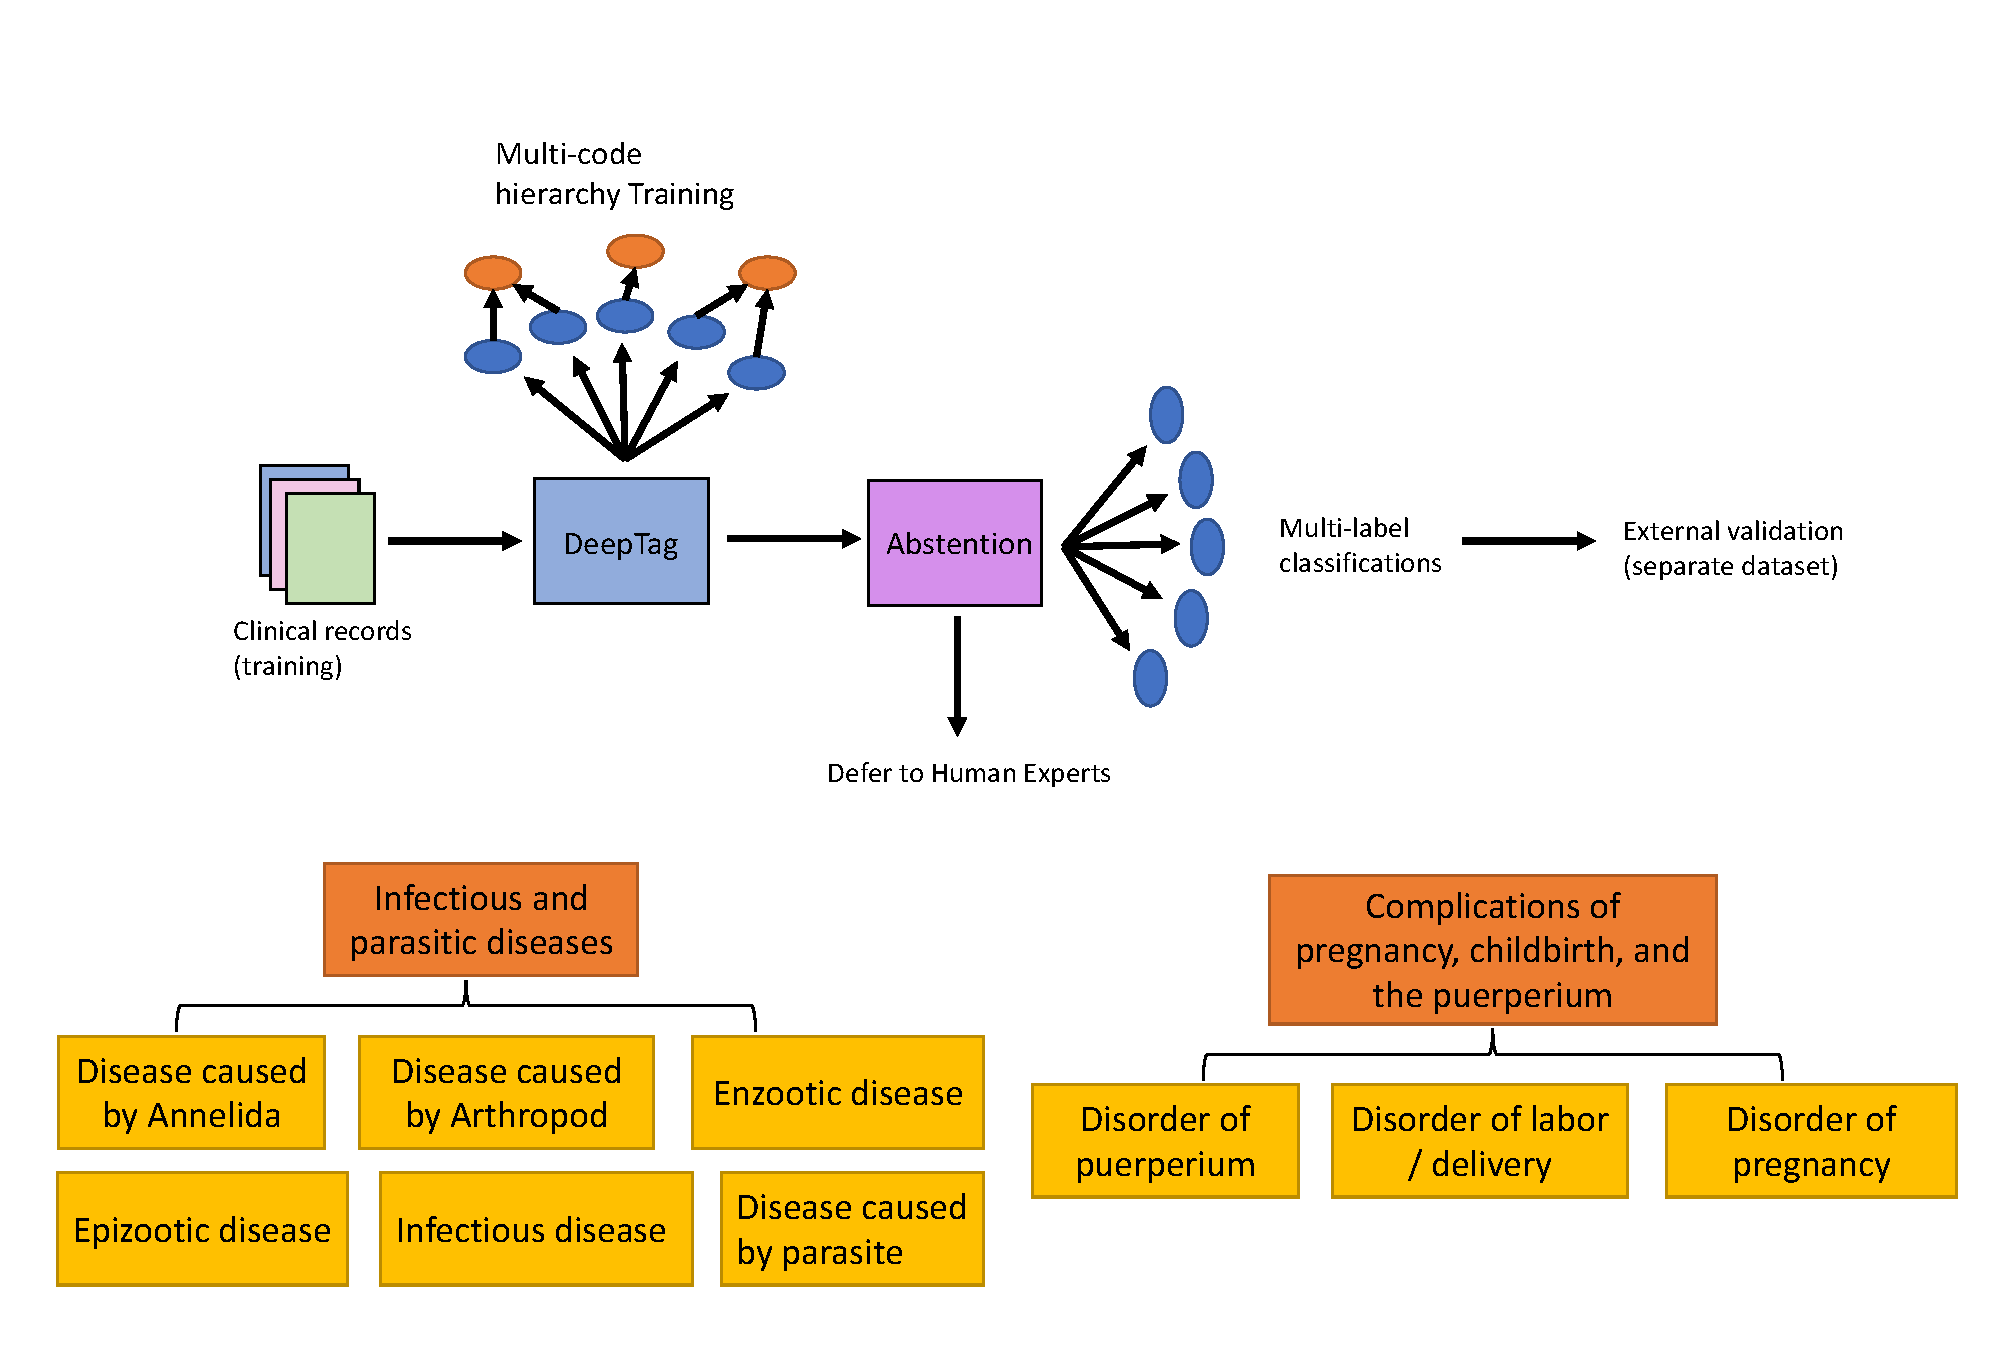
\includegraphics[scale=0.4]{combined-figure-1.pdf}
%         \caption{}
%         \label{fig:work-schematic}
%     \end{subfigure}
%     \hfill
%     \begin{subfigure}[b]{\textwidth}
%         \footnotesize
%         \textbf{CSU clinical note example}
%         \begin{framed}
%         Jem is a 10 year old male castrated hound mix that was presented for continuation of chemotherapy for previously diagnosed B-cell multicentric lymphoma. Jem was started on CHOP chemotherapy last week and has been doing very well since receiving doxorubicin. The owners have noted his lymph nodes have gotten much smaller. He has some loose stool, yet improved with metronidazole. Current medications include prednisolone. Assessment: Jem is in a strong partial remission based on today's physical exam. He is also doing very well since starting chemotherapy. A CBC today was unremarkable and adequate for chemotherapy. She was dispensed oral cyclophosphamide and furosemide that the owners were instructed to give at home.
%         \vspace{0.1in}
        
%         \textbf{Expert annotated diseases}: Disorder of hematopoietic cell proliferation, Neoplasm and/or hamartoma
%         % Disease codes: Disorder of hematopoietic cell proliferation(28), Neoplasm and/or hamartoma(40)
%         \end{framed}
        
%         \textbf{Private practice (PP) clinical note example}
%         \begin{framed}
%         Likely ear infection  shaking head  now swollen  drooping ear otherwise doing well  amublating well- had RF carpal arthrodesis at UCD. wt:  95.3 lbs.    Ears/Eyes/Nose/Throat: Clear OU/ brown yeasty debris AU errythema AU no fb/tm;s intact AU mod aural hematoma AD  Cardiovascular:   No murmur/arrhythmia.  Femoral pulses strong and synchronous. HR:84  Respiratory:  Lungs sound clear bilaterally  no crackles or wheezes. Eupneic.  RR:20  Lymph nodes:   No palpable peripheral lymphadenopathy  Oral Exam:  mm pink and moist.   CRT $<$ 2 sec  Musculoskeletal:  No lameness noted. Arthrodesis carpal joint RF  thickened stifle LH  ambulating well  Nervous System:   Appropriate mentation.  No overt neurologic deficits  Integument:  Full haircoat. Adequate skin turgor. otitis externa AU  aural hematoma AD. Ear cytology -  ++cocci  yeast   AU.  Cleaned  with epiotic. Rx Tresaderm BID x  14 days.  applied first dose    Rx temarilP taper    Skin prep medial AD over hematoma.  then 19g butterfly needle attached to syringe  drained 10ml bloody fluid  held pressure with guaze  no more bleeding        CE: Recheck in 14d to ensure infection cleared  discussed aural hematomas  options for tx  sx. may recur. 
%         \vspace{0.1in}
    
%         \textbf{Expert annotated diseases}: Infectious disease, Disorder of the integument, Disorder of the auditory system
%         \end{framed}
%         \caption{}
%         \label{fig:csu-pp-text-examples}
%     \end{subfigure}
%     \caption{{\bf System workflow and clinical note examples.} Figure (a) shows  the workflow of DeepTag  with abstention. Then we show two example meta-diseases corresponding to two subsets of the 42 SNOMED-CT codes. Figure (b) shows two example notes from the CSU and PP datasets. }
%     \label{fig:figure1}
% \end{figure*}

% \begin{figure}[!h]
% \centering
% 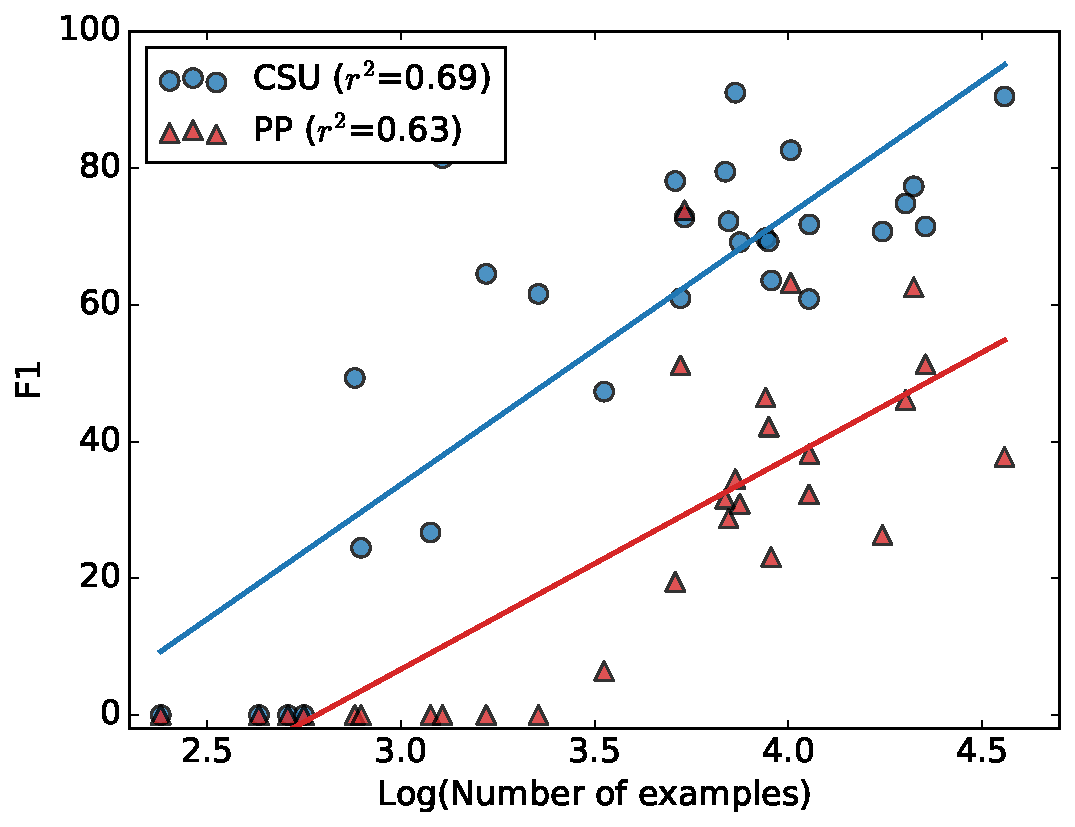
\includegraphics[scale=0.4]{example_f1_scatterplot.pdf}
% \caption{{\bf Per-disease code $F_1$ score plotted with log of number of examples in the training dataset.} Results shown here are from the DeepTag model. Each point represents a disease code, its corresponding number of training examples in CSU, and the per-disease code $F_1$ score from the DeepTag model.
% }
% \label{fig:example-f1-scatterplot}
% \end{figure}

% \begin{figure}[!t]
% \centering
% 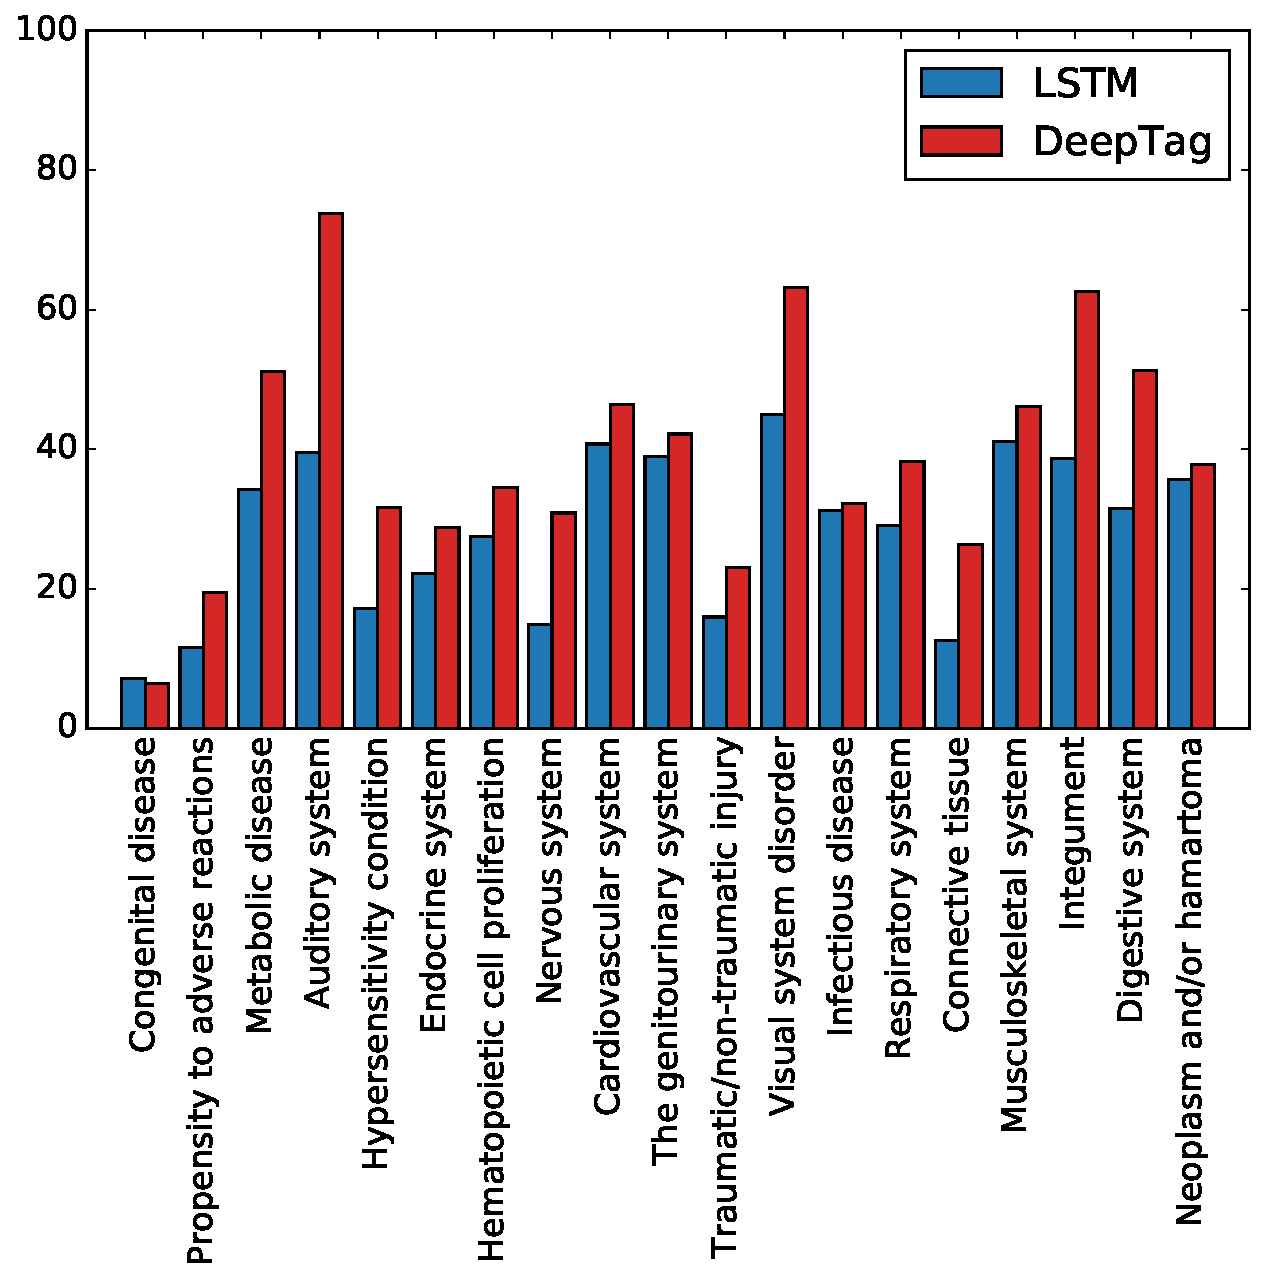
\includegraphics[scale=0.35]{performance-comparison-barplot.pdf}
% \caption{{\bf Performance comparison on PP.} 
% We compare the per-disease code $F_1$ score between baseline LSTM model and DeepTag model on the PP dataset. The disease codes are sorted from the least frequent to the most frequent in the training dataset, which comes from CSU.}
% \label{fig:pp-comparisons-barplot}
% \end{figure}

% \begin{figure}[!h]
%     \centering
%     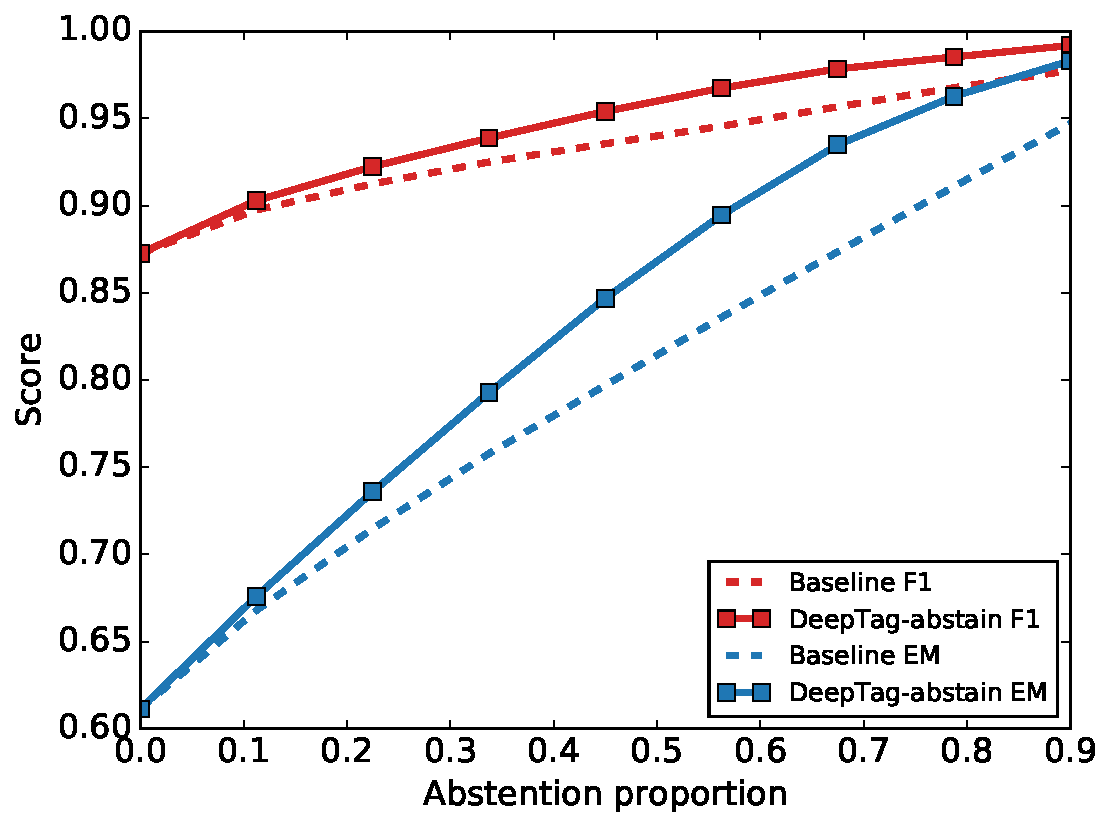
\includegraphics[scale=0.4]{best-abstainsion-2-deeptag.pdf}
% \caption{{\bf Comparison of the abstention models. } DeepTag-abstain is the abstention priority score estimator that uses confidence scores as input and estimate per-document accuracy of a given document. Baseline refers to the abstention scheme where the per-document abstention priority score is computed from individual disease code confidence scores without any learning. As a greater proportion of the examples are abstained from, the performance---$F_1$ and Exact Match (EM)---of both methods improve. DeepTag-abstain shows faster improvement, indicating that it learns to abstain in more difficult cases.}
% \label{fig:abs-best-curve}
% \end{figure}

% \begin{figure*}[!h]
% \centering
% 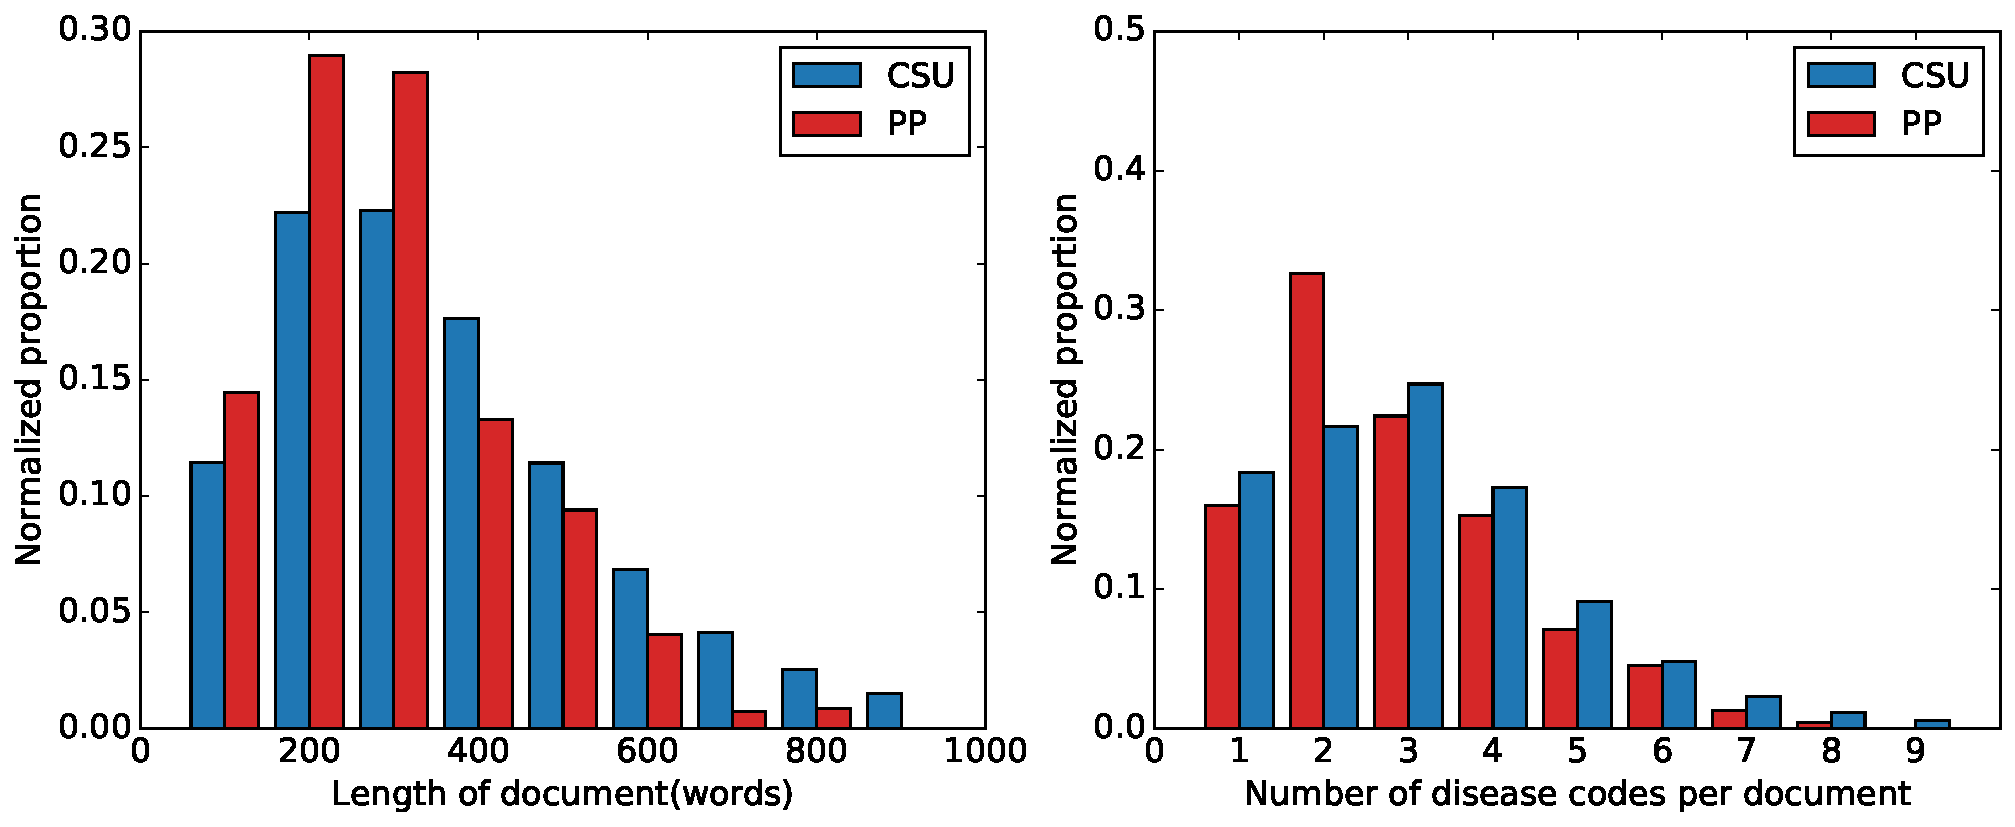
\includegraphics[scale=0.35]{doc-lengths-label-dist.pdf}
% \caption{{\bf Document length and disease code distribution on CSU and PP dataset.} 
% Proportion of records in each dataset with certain length (number of words) or certain number of disease codes.}
% \label{fig:doc-lengths-label-dist}
% \end{figure*}

% \clearpage

% \subsection*{Supplementary Tables}

% \begin{table*}[h]
% \centering
% \footnotesize
% \begin{adjustwidth}{-0.5in}{0in}
% \caption{\textbf{Report of DeepTag performance on the CSU test data and PP data}}
% \begin{tabular}{c | c c c c c c | c c c c c c }
% \toprule
%  & \multicolumn{6}{c|}{CSU} & \multicolumn{6}{c}{PP (Cross-hospital)}  \\
% Disease code & N & Prec & Rec & $F_1$ & AUC & Sub & N & Prec & Rec & $F_1$ & AUC & Sub \\
% \midrule
% Autoimmune disease & 1280 & 94.0 & 72.3 & 81.4 & 0.86 & 11 & 1 & 0.0 & 0.0 & 0.0 & 0.50 & 1(1) \\
% Congenital disease & 3345 & 72.9 & 35.9 & 47.3 & 0.68 & 224 & 17 & 46.7 & 3.5 & 6.4 & 0.52 & 8(6) \\
% Propensity to adverse reactions & 5105 & 89.1 & 70.2 & 78.1 & 0.85 & 8 & 43 & 67.2 & 12.6 & 19.5 & 0.56 & 7(2) \\
% Metabolic disease & 5265 & 68.9 & 55.4 & 61.0 & 0.77 & 82 & 26 & 56.6 & 48.5 & 51.1 & 0.73 & 12(9) \\
% Disorder of auditory system & 5393 & 81.0 & 66.2 & 72.8 & 0.83 & 67 & 64 & 78.8 & 70.3 & 73.8 & 0.84 & 12(6) \\
% Hypersensitivity condition & 6871 & 85.7 & 74.6 & 79.5 & 0.87 & 31 & 50 & 67.7 & 22.4 & 31.6 & 0.61 & 11(4) \\
% Disorder of endocrine system & 7009 & 79.2 & 66.7 & 72.2 & 0.83 & 84 & 46 & 44.4 & 21.7 & 28.7 & 0.60 & 8(8) \\
% Disorder of hematopoietic cell proliferation & 7294 & 95.1 & 87.4 & 91.0 & 0.94 & 22 & 16 & 62.7 & 25.0 & 34.5 & 0.62 & 6(1) \\
% Disorder of nervous system & 7488 & 76.1 & 63.8 & 69.2 & 0.81 & 243 & 27 & 40.4 & 26.7 & 30.8 & 0.62 & 19(14) \\
% Disorder of cardiovascular system & 8733 & 79.3 & 62.5 & 69.7 & 0.81 & 351 & 53 & 44.1 & 52.1 & 46.4 & 0.73 & 30(24) \\
% Disorder of the genitourinary system & 8892 & 77.7 & 62.6 & 69.3 & 0.81 & 317 & 44 & 47.8 & 39.1 & 42.2 & 0.68 & 19(12) \\
% Traumatic AND/OR non-traumatic injury & 9027 & 72.8 & 57.2 & 63.5 & 0.78 & 536 & 19 & 50.5 & 15.8 & 23.1 & 0.58 & 13(8) \\
% Visual system disorder & 10139 & 84.3 & 81.1 & 82.6 & 0.90 & 413 & 62 & 65.0 & 62.6 & 63.2 & 0.79 & 39(34) \\
% Infectious disease & 11304 & 71.2 & 53.7 & 60.8 & 0.76 & 260 & 88 & 63.8 & 23.0 & 32.3 & 0.60 & 20(10) \\
% Disorder of respiratory system & 11322 & 79.5 & 65.5 & 71.8 & 0.82 & 274 & 27 & 38.3 & 42.2 & 38.2 & 0.69 & 16(14) \\
% Disorder of connective tissue & 17477 & 75.4 & 67.0 & 70.7 & 0.81 & 567 & 24 & 30.4 & 24.2 & 26.3 & 0.61 & 15(11) \\
% Disorder of musculoskeletal system & 20060 & 77.0 & 73.4 & 74.8 & 0.84 & 670 & 56 & 54.0 & 41.4 & 46.1 & 0.69 & 31(19) \\
% Disorder of integument & 21052 & 84.2 & 71.6 & 77.3 & 0.84 & 360 & 156 & 65.7 & 60.1 & 62.6 & 0.74 & 58(32) \\
% Disorder of digestive system & 22589 & 76.8 & 67.1 & 71.5 & 0.81 & 694 & 195 & 58.0 & 47.9 & 51.3 & 0.65 & 47(36) \\
% Neoplasm and/or hamartoma & 36108 & 92.2 & 88.9 & 90.5 & 0.93 & 749 & 59 & 26.1 & 72.5 & 37.8 & 0.74 & 18(7) \\
% \bottomrule
% \end{tabular}
% \begin{flushleft} This table reports the DeepTag's performance (precision, recall, $F_1$ and AUC) for the 20 most frequent disease codes (from a total of 42 disease codes). $N$ indicates the total number of examples in the dataset. AUC refers to area under the receiver operator curve. Sub indicates the number of lower-level disease codes that are present in the dataset that are binned into one of the disease level codes. For the PP dataset, the Sub number in parentheses indicate the number of subtypes that are also present in CSU dataset. 
% \end{flushleft}
%  \label{tab:detailed-csu-pp}
% \end{adjustwidth}
% \end{table*}

% \begin{table*}[!h]
% \centering
% \footnotesize
% \caption{\textbf{Evaluation of  trained classifiers on the CSU and PP data}}
% \begin{tabular}{c | c | c c | c c | c c }
% \toprule
% Model & \multicolumn{1}{c|}{EM} & \multicolumn{2}{c|}{Precision} & \multicolumn{2}{c|}{Recall} & \multicolumn{2}{c}{$F_1$} \\
% & & unwgt & wgt & unwgt & wgt & unwgt & wgt \\
% \midrule
% & \multicolumn{7}{c}{CSU data} \\
% \midrule
% MetaMap - SVM & 32.2 & 52.2 & 74.8 & 54.8 & 75.0 & 53.2 & 74.8 \\
% MetaMap - MLP & 41.2 & 64.7 & 82.6 & 48.5 & 71.8 & 55.0 & 76.4 \\
% CNN & 45.1 & 73.1 & 84.4 & 57.2 & 78.4 & 62.2 & 80.9 \\
% LSTM & 47.4 & 76.6 & 85.9 & 59.3 & 78.7 & 65.3 & 81.7 \\ 
% BLSTM & 48.2 & 76.1 & 86.0 & 57.6 & 79.4 & 63.5 & 82.2 \\ 
% DeepTag-M & \textbf{48.6} & 76.8 & \textbf{86.3} & 58.7 & 79.6 & 64.6 & 82.4 \\
% \textbf{DeepTag} & 48.4 & \textbf{79.9} & 86.1 & \textbf{62.1} & \textbf{79.8} & \textbf{68.0} & \textbf{82.4} \\ 
% \midrule
% \midrule
% & \multicolumn{7}{c}{PP data (Cross-hospital)} \\
% \midrule
% MetaMap - SVM & 3.2 & 26.5 & 57.3 & 37.7 & 53.1 & 24.8 & 51.6 \\
% MetaMap - MLP & 13.8 & 30.6 & 56.4 & 24.9 & 47.7 & 26.2 & 50.5 \\
% CNN & 13.5 & 52.8 & 68.5 & 31.8 & 54.0 & 34.8 & 56.0 \\
% LSTM & 13.8 & 48.1 & 65.7 & 31.8 & 51.9 & 33.8 & 54.4 \\ 
% BLSTM & 13.8 & 47.3 & 66.0 & 35.6 & 57.9 & 36.9 & 58.4 \\ 
% DeepTag-M & 17.1 & 53.4 & 68.0 & 37.9 & 59.9 & 40.6 & 61.1 \\ 
% \textbf{DeepTag} & \textbf{17.4} & \textbf{56.5} & \textbf{70.3} & \textbf{41.4} & \textbf{62.4} & \textbf{43.2} & \textbf{63.4} \\ 
% \bottomrule
% \end{tabular}
% \begin{flushleft}
% Aggregate prediction performance across the 42 disease codes. 
% We trained a multi-layer perceptron (MetaMap-MLP) algorithm and support vector machines (MetaMap-SVM) algorithm on discrete features generated by the MetaMap, which processes a document and extracts medically-relevant terms~\cite{aronson2010overview}.
% CNN refers to a text convolution neural network implementation from Kim~\cite{kim2014convolutional}. BLSTM refers to the multi-task bidirectional LSTM. DeepTag is our best model, and DeepTag-M is the variation with a meta-disease loss. EM indicates the exact match ratio, which is the percentage of the clinical notes where the algorithm perfectly predicts all of the disease codes. For example, if a note has three true disease codes, then the algorithm achieves an exact match if it predicts exactly these three disease codes, no more and no less. For each precision, recall and $F_1$ score, there are two ways to compute an algorithm's performance. First we can take an unweighted average of the score across all the disease codes (unwgt) or we can take an average weighted by the number of test examples in each disease code (wgt). All the algorithms are trained on CSU and tested on a held-out CSU data and the PP data. 
% \end{flushleft}
%  \label{tab:pp}
% \end{table*}

% Figures and tables can be referenced in LaTeX using the ref command, e.g. Figure \ref{fig:stream} and Table \ref{tab:example}.

\end{document}